\section{Architecture}
\label{sec:architecture}
%% ============================================================

\Beluga{} is an L3 chain in the \Lux{} layered architecture:

\begin{center}
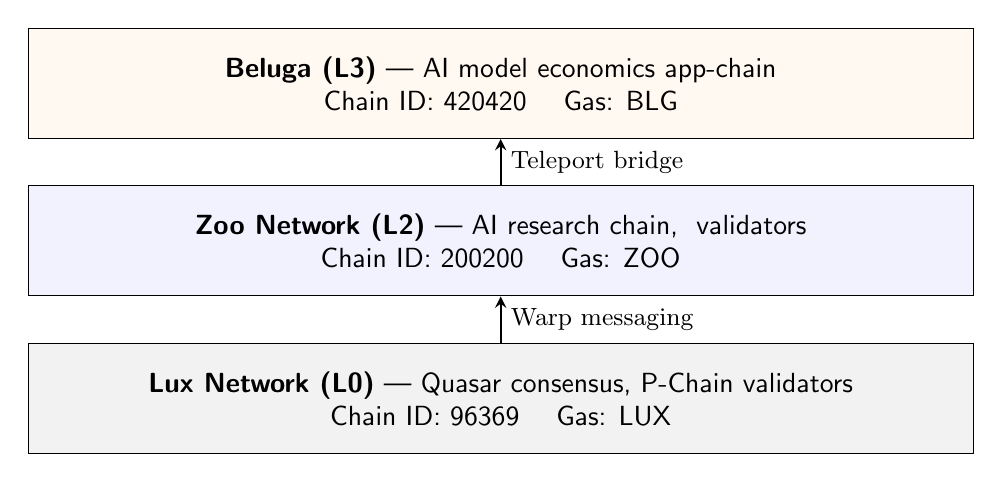
\begin{tikzpicture}[
    layer/.style={rectangle, draw, minimum width=12cm, minimum height=1.4cm, align=center, font=\sffamily},
    arr/.style={->, thick, >=stealth}
]
\node[layer, fill=black!5] (l0) at (0,0) {\textbf{Lux Network (L0)} --- Quasar consensus, P-Chain validators\\Chain ID: 96369 \quad Gas: LUX};
\node[layer, fill=blue!5] (l2) at (0,2) {\textbf{Zoo Network (L2)} --- AI research chain, \Zoo{} validators\\Chain ID: 200200 \quad Gas: ZOO};
\node[layer, fill=orange!5] (l3) at (0,4) {\textbf{Beluga (L3)} --- AI model economics app-chain\\Chain ID: 420420 \quad Gas: BLG};

\draw[arr] (l0) -- (l2) node[midway, right, font=\small] {Warp messaging};
\draw[arr] (l2) -- (l3) node[midway, right, font=\small] {Teleport bridge};
\end{tikzpicture}
\end{center}

\subsection{Layer Responsibilities}

\begin{description}[leftmargin=2cm, style=nextline]
    \item[Lux (L0)] Provides the base consensus layer via Quasar 3.0 \cite{lux-quasar} (Lux LP-020), a post-HotStuff BFT protocol with post-quantum security and sub-second finality at $O(n)$ message complexity. All validator sets are anchored on the P-Chain. Warp messaging enables verified cross-chain communication between any two Lux chains. \Beluga{} settlement and \Zoo{} per-LLM chains \cite{zoo-per-llm-chains} share this base.
    \item[Zoo (L2)] A research-focused EVM chain (chain ID 200200) with ZOO as the native gas token. Zoo hosts the Agent NFT standard \cite{zoo-agent-nft}, the Experience Ledger \cite{zoo-experience-ledger}, and the \DSO{} adaptation framework \cite{zoo-dso}. Zoo validators run the \texttt{zood} binary, which is a superset of \texttt{luxd} with AI-specific extensions.
    \item[Beluga (L3)] An application-specific chain with its own block production, state, and gas token. \Beluga{} inherits Zoo's validator set---no new node binary is required. Validators that run \texttt{zood} automatically validate \Beluga{} blocks via the same process that validates Zoo subnets.
\end{description}

\subsection{Block Production}

\Beluga{} produces blocks independently of \Zoo{}, with the following parameters:

\begin{table}[h]
\centering
\caption{Beluga chain parameters.}
\label{tab:params}
\begin{tabular}{@{}ll@{}}
\toprule
Parameter & Value \\
\midrule
Chain ID & 420420 \\
Block time & 500ms \\
Gas limit & 30M per block \\
Gas token & BLG (18 decimals) \\
EVM version & Shanghai \\
Consensus & PoAI-adapted Quasar \\
Validator set & Inherited from Zoo \\
Finality & $\leq 1.1$s (2 blocks + attestation) \\
\bottomrule
\end{tabular}
\end{table}

\subsection{Cross-Chain Communication}

\Beluga{} uses two bridging mechanisms:

\begin{enumerate}
    \item \textbf{Teleport} (Beluga $\leftrightarrow$ Zoo): Native \Lux{} Teleport bridge \cite{lux-teleport} for BLG/ZOO token transfers. Teleport uses BLS aggregate signatures from the shared validator set, achieving trustless bridging without external relayers.
    \item \textbf{Warp} (Beluga $\leftrightarrow$ any Lux chain): General-purpose cross-chain messaging via Lux Warp Messaging for arbitrary contract calls, model metadata queries, and experience ledger lookups.
\end{enumerate}

%% ============================================================
